%% The following macros taken from the CMS note
%\wip{Text to be updated to reflect ATLAS+CMS combination. Maybe show only S2}

In this section combination results are given for a parametrisation based on the coupling modifier, or $\kappa$-framework~\cite{Heinemeyer:2013tqa}. A set of coupling modifiers, $\vec\kappa$, is introduced to parametrize potential deviations from the SM~predictions of the Higgs boson couplings to SM~bosons and fermions. For a given production process or decay mode $j$, a coupling modifier $\kappa_j$ is defined such that,

\begin{equation}
\label{eq:kappa}
  \kappa_j^2=\sigma_j/\sigma_j^\SM\ \ \ {\rm or}\ \ \  \kappa_j^2=\Gamma^j/\Gamma^j_\SM.
\end{equation}

In the SM, all $\kappa_j$ values are positive and equal to unity. Six coupling modifiers corresponding to the tree-level Higgs boson couplings are defined: $\kW$, $\kZ$, $\ktop$, $\kb$, $\ktau$ and $\kmu$. In addition, the effective coupling modifiers $\kglu$, $\kgam$ and $\kzgam$ are introduced to describe \ggh production, \hgg decay and \hzg decay loop processes. 
The total width of the Higgs boson, relative to the SM prediction, varies with the coupling modifiers as $\GammaSM = \sum_{j}\mathrm{B}^{j}_{\text{SM}}\kappa_{j}^{2} / (1 - \Bbsm)$, where $\mathrm{B}^{j}_{\text{SM}}$ is the SM branching fraction for the $\PH\rightarrow jj$ channel and $\Bbsm$ is the Higgs boson branching fraction to BSM final states. In the results for the $\kappa_j$ parameters presented here $\Bbsm$ is fixed to zero and only decays to SM particles are allowed. Projections are also given for the upper limit on $\Bbsm$ when this restriction is relaxed, in which an additional constraint that $|\kV| < 1$ is imposed. 
%A constraint on $\GammaSM$ is also obtained in this model by treating it as a free parameter in place of one of the other $\kappa$ parameters.

The expected uncertainties for the coupling modifier parametrization for ATLAS, CMS~\cite{ATLAS-PHYS-PUB-2018-XY,CMS-PAS-FTR-18-011} and their combination for scenario S2 are summarized in Figure~\ref{fig:summary_K2} while the numerical values are provided in Table~\ref{tab:summary_K2}.
For the combined measurement in S2, the uncertainty components  contribute at a similar level for $\kgam$, $\kW$, $\kZ$ and $\ktau$. The signal theory remains the main component for $\ktop$ and $\kglu$, while $\kmu$ and $\kzgam$ are limited by statistics.

The expected uncertainties on $\Bbsm$ and $\GammaSM$ for the parametrisation with $\Bbsm\geq0$ and $|\kV|\leq1$. The $1\sigma$ uncertainty on $\Bbsm$ is $0.035$ ($0.048$) in S1 and $0.027$ ($0.032$) in S2 for CMS (ATLAS), where in the latter case the statistical uncertainty is the largest component.
The expected uncertainty for the ATLAS-CMS combination on  $\Bbsm$ is XXXX in S2. 
%The corresponding 95\% CL expected upper limit is $\Bbsm = 0.077 (0.057)$ in S1 (S2). The uncertainty on $\GammaSM$ is $0.05$ in S1 and $0.04$ in S2, equivalent to $0.16$ and $0.21\UMeV$ respectively, assuming the SM width of $4.1\UMeV$. The main contribution is the statistical uncertainty, followed by the experimental one.

\begin{figure}[hbtp]
\centering
% \includegraphics[width=0.5\textwidth]{\main/section2/plots/comb/summary_K2_300.pdf}%
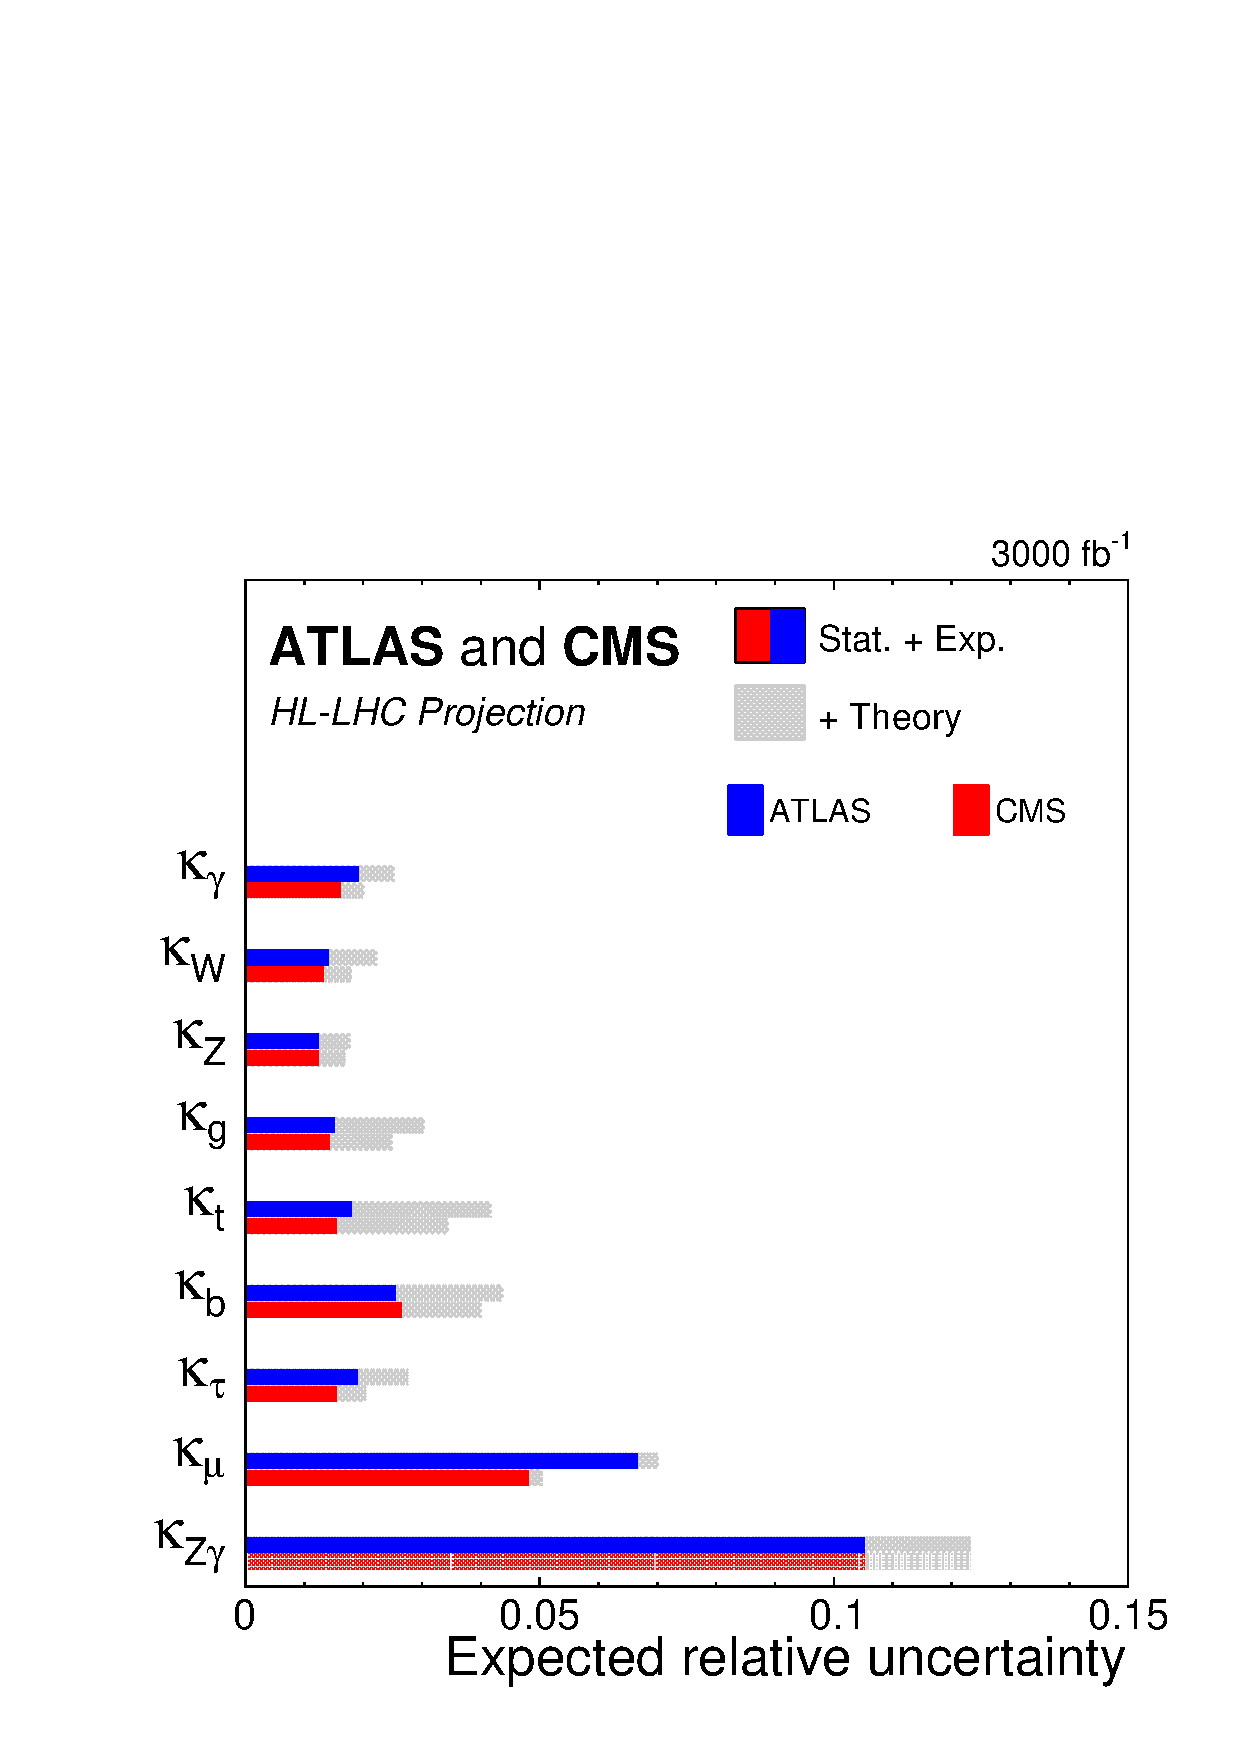
\includegraphics[width=0.48\textwidth]{\main/section2/plots/comb/yr_combined_summary_K2_3000.pdf}%
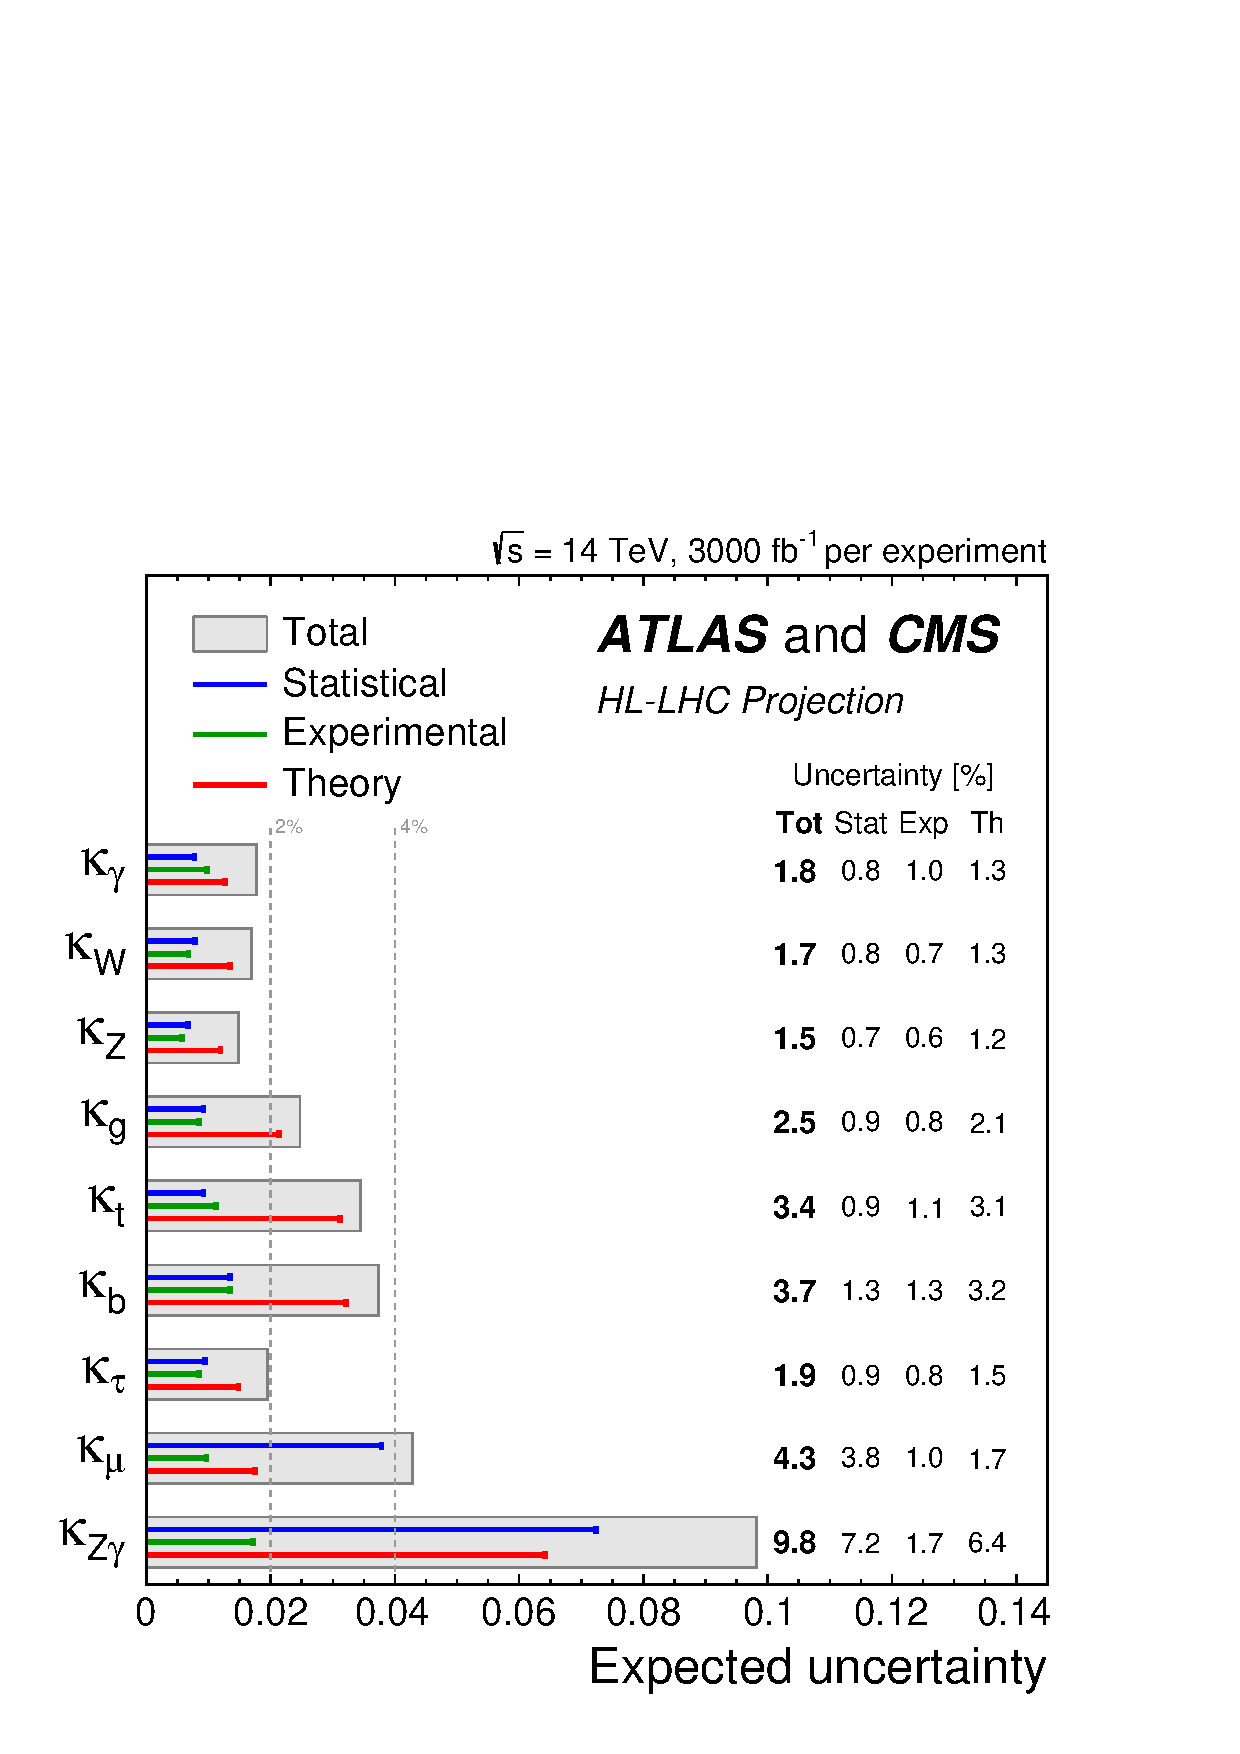
\includegraphics[width=0.48\textwidth]{\main/section2/plots/comb/final_k2_diag_v2.pdf}%
\caption{(left) Summary plot showing the total expected $\pm 1\sigma$ uncertainties in S2 (with YR18 systematic uncertainties) on the coupling modifier parameters   for ATLAS (blue)  and CMS (red). The filled coloured box corresponds to the statistical and experimental systematic uncertainties, while the hatched grey area represent the additional contribution to the total uncertainty due to theoretical systematic uncertainties.
(right) Summary plot showing the total expected $\pm 1\sigma$  uncertainties in S2 (with YR18 systematic uncertainties) on the coupling modifier parameters for the combination of ATLAS and CMS extrapolations. For each measurement,  the total uncertainty is indicated by a grey box while the statistical, experimental and theory uncertainties are indicated by a blue, green and red line respectively.}
%\caption{Summary plot showing the total expected $\pm 1\sigma$ uncertainties in S1 (with Run~2 systematic uncertainties~\cite{Sirunyan:2018koj}) and S2 (with YR18 systematic uncertainties) on the coupling modifier parameters. The statistical-only component of the uncertainty is also shown.}
\label{fig:summary_K2}
\end{figure}


\begin{table}[hbtp]
\centering
\caption{The expected $\pm 1\sigma$ uncertainties, expressed as percentages, on the coupling modifier parameters.%, as well as $\Bbsm$ and $\GammaSM$. Due to the constraint $\Bbsm \geq 0$ the values for this parameter correspond to the $+1\sigma$ uncertainties only.
Values are given for both S1 (with Run~2 systematic uncertainties~\cite{Sirunyan:2018koj}) and S2 (with YR18 systematic uncertainties). The total uncertainty is decomposed into four components: statistical (Stat), signal theory (SigTh), background theory (BkgTh) and experimental (Exp).\wip{to add comb results for S2 as well}}
\small
\begin{tabular}{@{} l c c@{\hskip 0.15in} c c c c @{}}
  \hline
     \multicolumn{7}{c}{ATLAS}\\
 \hline
  &  & \multicolumn{5}{c}{3000 $\text{fb}^{-1}$} \\
  &  & Total & Stat & SigTh & BkgTh & Exp \\
  \hline
  \multirow{2}{*}{$\kappa_{\gamma }$} & S1 & 3.7   & 0.9   & 2.2   & 1.4   & 2.5  \\[1pt]
  & S2& 2.4   & 0.9   & 1.1   & 0.9   & 1.7  \\[4pt]
  \multirow{2}{*}{$\kappa_{\mathrm{W}}$} & S1  & 3.1   & 0.8   & 1.9   & 1.9   & 1.3  \\[1pt]
  & S2 & 2.2   & 0.8   & 1.2   & 1.3   & 1.2  \\[4pt]
  \multirow{2}{*}{$\kappa_{\mathrm{Z}}$} & S1 & 2.6   & 0.8   & 1.8   & 1.2   & 1.1  \\[1pt]
  & S2 & 1.8   & 0.8   & 1.0   & 0.8   & 0.9  \\[4pt]
  \multirow{2}{*}{$\kappa_{\mathrm{g}}$} & S1 & 4.2   & 1.0   & 3.2   & 2.2   & 1.4  \\[1pt]
  & S2 & 3.1   & 1.0   & 2.2   & 1.6   & 1.2  \\[4pt]
  \multirow{2}{*}{$\kappa_{\mathrm{t}}$} & S1 & 6.3   & 1.1   & 4.9   & 3.4   & 1.6  \\[1pt]
  & S2 & 4.2   & 1.1   & 2.6   & 2.7   & 1.4  \\[4pt]
  \multirow{2}{*}{$\kappa_{\mathrm{b}}$} & S1 & 6.2   & 1.6   & 3.7   & 4.1   & 2.3  \\[1pt]
  & S2  & 4.4   & 1.6   & 2.1   & 2.8   & 2.0  \\[4pt]
  \multirow{2}{*}{$\kappa_{\tau }$} & S1 & 3.7 & 1.1   & 2.6   & 1.8   & 1.7  \\[1pt]
  & S2 & 2.7   & 1.1   & 1.5   & 1.2   & 1.6  \\[4pt]
  \multirow{2}{*}{$\kappa_{\mu}$} & S1  & 7.7 & 6.4   & 3.6   & 1.4   & 1.9  \\[1pt]
  & S2 & 7.0   & 6.4   & 2.0   & 0.9   & 1.8  \\[4pt]
  \multirow{2}{*}{$\kappa_{\mathrm{Z}\gamma}$} & S1 & 12.7  & 10.2  & 6.9   & 1.4   & 2.5  \\[1pt]
  & S2 & 12.4  & 10.2  & 6.4   & 0.9   & 2.4  \\[4pt]
  \hline
\end{tabular}
\hspace{0.5cm}
\begin{tabular}{@{} l c c@{\hskip 0.15in} c c c c @{}}
 \hline
   \multicolumn{7}{c}{CMS}\\
 \hline
  &  & \multicolumn{5}{c}{3000 $\text{fb}^{-1}$} \\
  &  & Total & Stat & SigTh & BkgTh & Exp \\
 \hline
\multirow{2}{*}{$\kappa_{\gamma }$} & S1  & 2.9& 1.1 & 1.8 & 1.0 & 1.7  \\[1pt]
                        & S2  & 2.0& 1.1 & 0.9 & 0.8 & 1.2  \\[4pt]
\multirow{2}{*}{$\kappa_{\mathrm{W}}$} & S1  & 2.6& 1.0 & 1.7 & 1.1 & 1.1  \\[1pt]
                        & S2  & 1.8& 1.0 & 0.9 & 0.8 & 0.8  \\[4pt]
\multirow{2}{*}{$\kappa_{\mathrm{Z}}$} & S1  & 2.4& 1.0 & 1.7 & 0.9 & 0.9  \\[1pt]
                        & S2  & 1.7& 1.0 & 0.9 & 0.7 & 0.7  \\[4pt]
\multirow{2}{*}{$\kappa_{\mathrm{g}}$} & S1  & 4.0& 1.1 & 3.4 & 1.3 & 1.2  \\[1pt]
                        & S2  & 2.5& 1.1 & 1.7 & 1.1 & 1.0  \\[4pt]
\multirow{2}{*}{$\kappa_{\mathrm{t}}$} & S1  & 5.5& 1.0 & 4.4 & 2.7 & 1.6  \\[1pt]
                        & S2  & 3.5& 1.0 & 2.2 & 2.1 & 1.2  \\[4pt]
\multirow{2}{*}{$\kappa_{\mathrm{b}}$} & S1  & 6.0& 2.0 & 4.3 & 2.9 & 2.3  \\[1pt]
                        & S2  & 4.0& 2.0 & 2.0 & 2.2 & 1.8  \\[4pt]
\multirow{2}{*}{$\kappa_{\tau }$} & S1  & 2.8& 1.2 & 1.8 & 1.1 & 1.4  \\[1pt]
                        & S2  & 2.0& 1.2 & 1.0 & 0.9 & 1.0  \\[4pt]
\multirow{2}{*}{$\kappa_{\mu}$} & S1  & 6.7& 4.7 & 2.5 & 1.0 & 3.9  \\[1pt]
                        & S2  & 5.0& 4.7 & 1.3 & 0.8 & 1.1  \\[4pt]
\hline
\end{tabular}
\label{tab:summary_K2}
\vspace{0.5cm}
\end{table}

%\wip{Correlation info maybe only textual}


%Figure~\ref{fig:corr_K2} gives the correlation coefficients for the coupling modifiers for S2. In contrast to the per-decay signal strength correlations in Figure~\ref{fig:corr_A1_5D} the correlations here are larger, up to $+0.74$. One reason for this is that the normalisation of any signal process depends on the total width of the Higgs boson, which in turn depends on the values of the other coupling modifiers. The largest correlations involve $\kb$, as this gives the largest contribution to the total width in the SM. Therefore improving the measurement of the $\hbb$ process will improve the sensitivity of many of the other coupling modifiers at the HL-LHC.

The correlation coefficients between the coupling modifiers are in general larger compared to the one related to the signal strength (up to $+XX$ ). One reason for this is that the normalisation of any signal process depends on the total width of the Higgs boson, which in turn depends on the values of the other coupling modifiers. The largest correlations involve $\kb$, as this gives the largest contribution to the total width in the SM. Therefore improving the measurement of the $\hbb$ process will improve the sensitivity of many of the other coupling modifiers at the HL-LHC.


%\begin{figure}[hbtp]
%\centering
% \includegraphics[width=0.5\textwidth]{\main/section2/plots/comb/correlations_K2_S2_300.pdf}%
%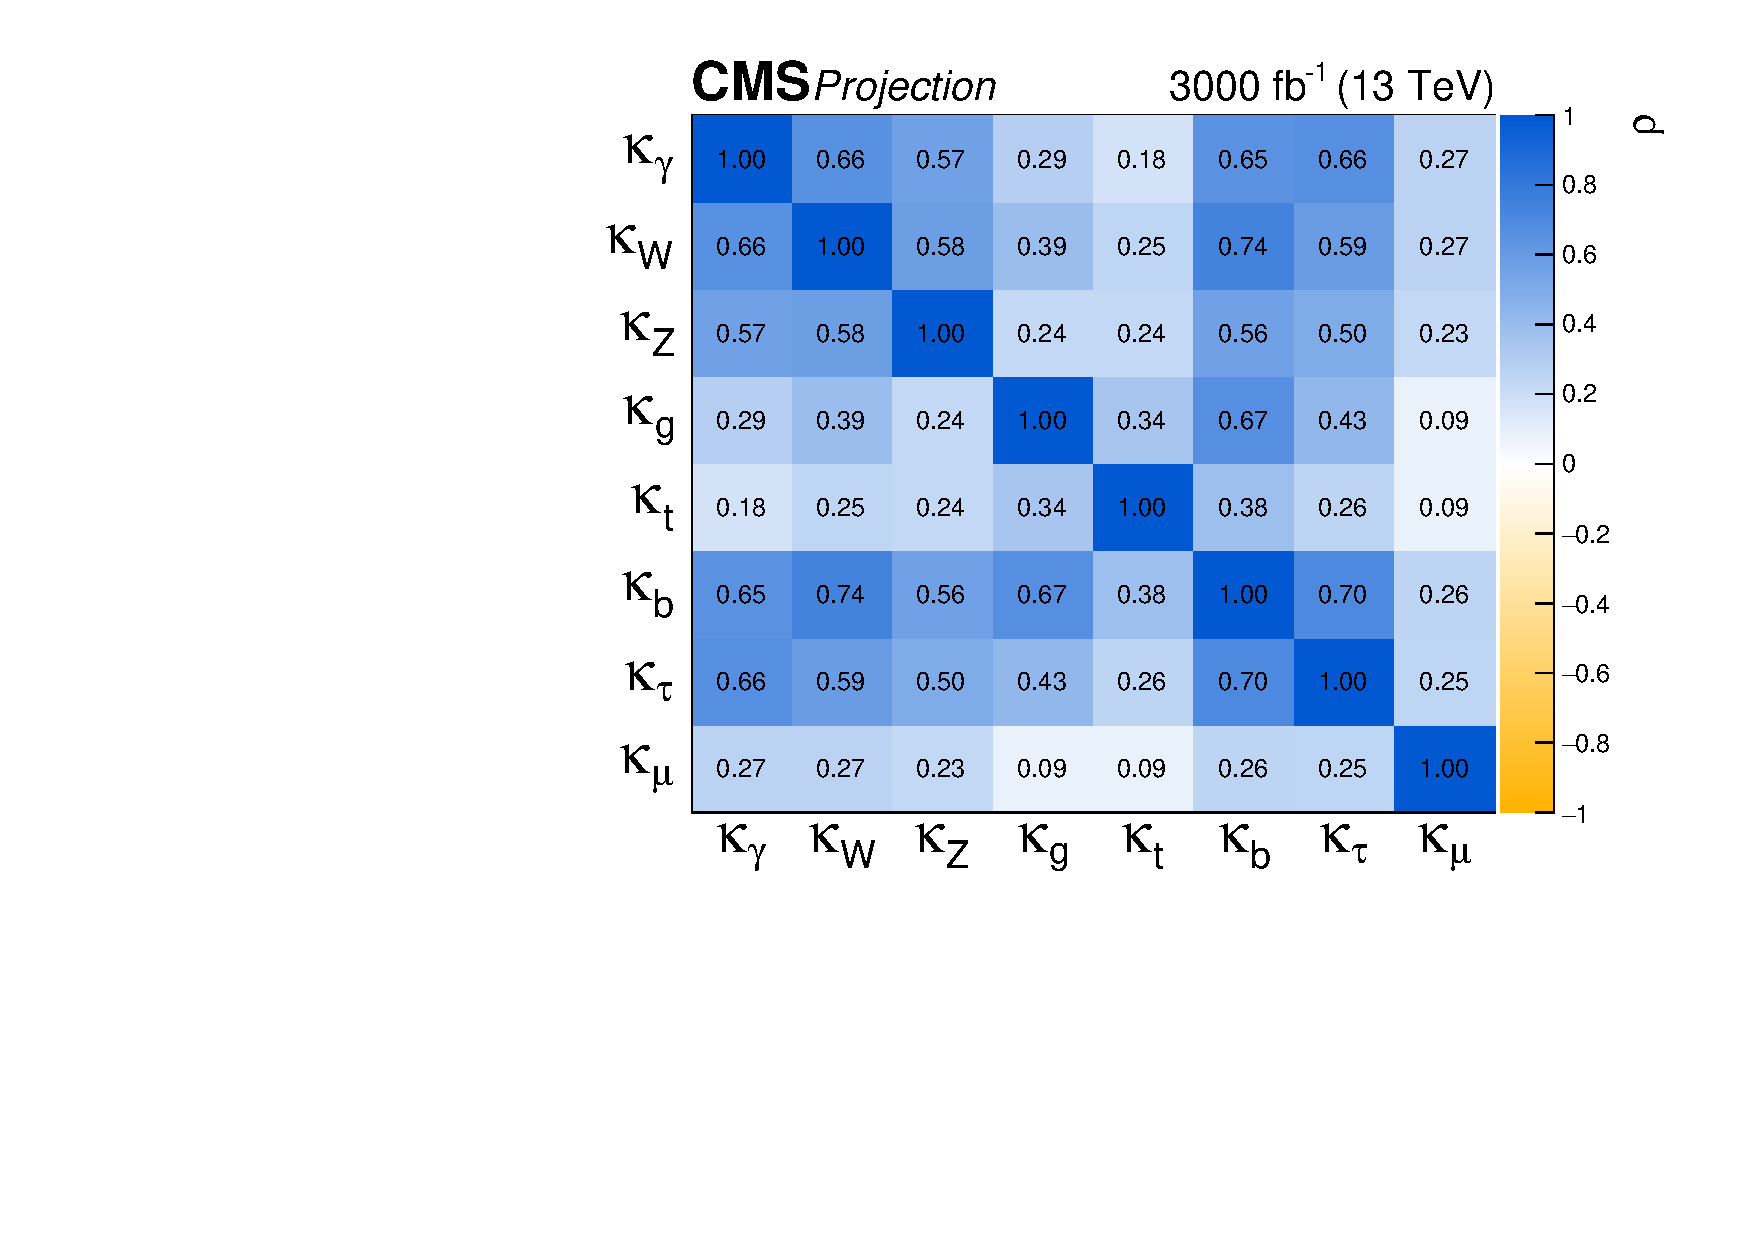
\includegraphics[width=0.6\textwidth]{\main/section2/plots/comb/correlations_K2_S2_3000.pdf}%
%\caption{Correlation coefficients ($\rho$) between parameters in the coupling modifier parametrisation for S2 (with YR18 systematic uncertainties).}
%\label{fig:corr_K2}
%\end{figure}

Projections have also been determined for a parametrisation based on ratios of the coupling modifiers ($\lambda_{ij} = \kappa_{i}/\kappa_{j}$) together with a reference ratio of coupling modifiers $\kappa_{gZ} = \kglu\kZ/\kH$.
This parametrization requires no assumption on the total width of the Higgs boson, as its effective modifier $\kH$ has been absorbed into the ratio $\kappa_{gZ}$. The results of this projection for ATLAS, CMS and their combination in S2 are given in Fig~\ref{fig:summary_L1}.
The numerical values for both S1 and S2 for the projections of the two experiments and their combination for S2 are given in Table~\ref{tab:summary_L1}.
\begin{figure}[hbtp]
\centering
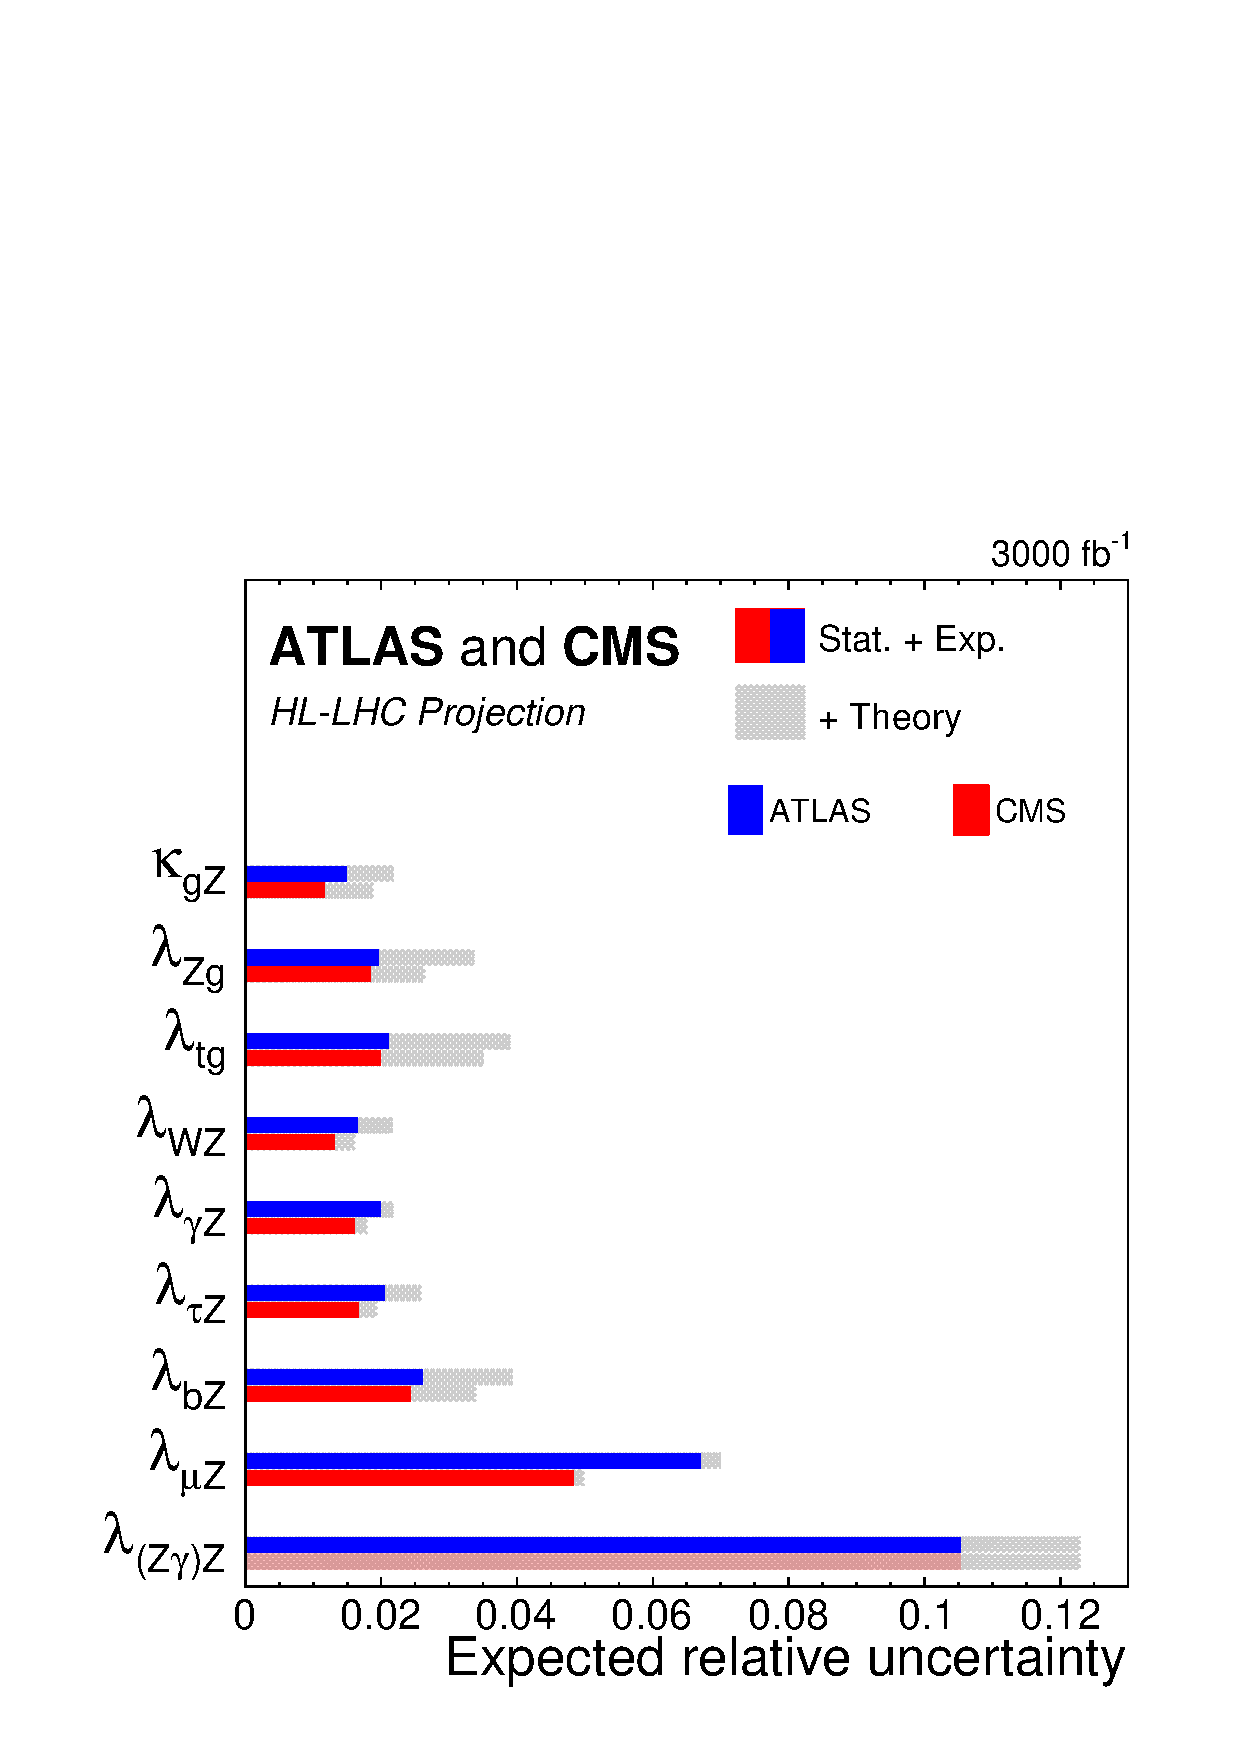
\includegraphics[width=0.48\textwidth]{\main/section2/plots/comb/yr_combined_summary_L1_3000.pdf}%
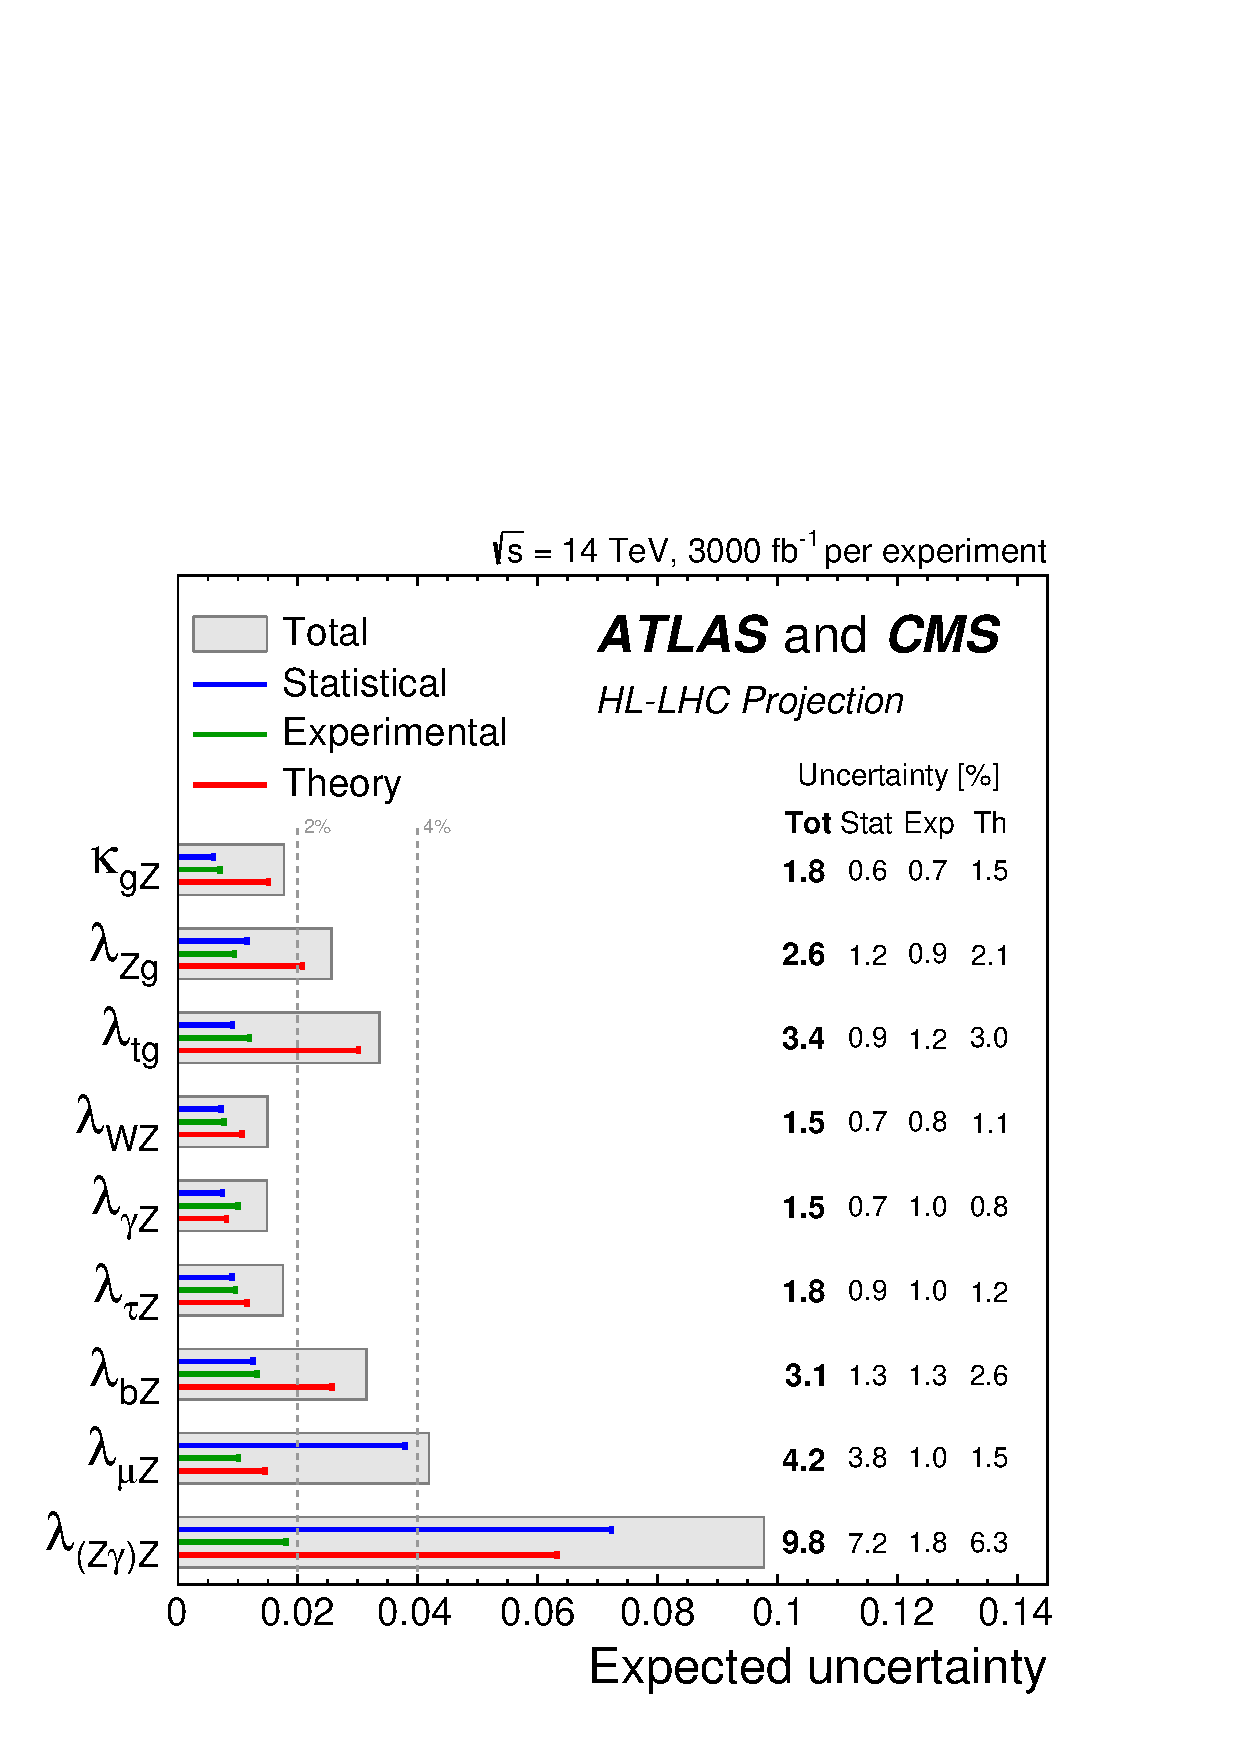
\includegraphics[width=0.48\textwidth]{\main/section2/plots/comb/yr_combined_L1.pdf}%
\caption{(left) Summary plot showing the total expected $\pm 1\sigma$ uncertainties in S2 (with YR18 systematic uncertainties) on the ratios of coupling modifier parameters  for ATLAS (blue)~\cite{ATLAS-PHYS-PUB-2018-XY} and CMS (red)~\cite{CMS-PAS-FTR-18-011}. The filled coloured box corresponds to the statistical and experimental systematic uncertainties, while the hatched grey area represent the additional contribution to the total uncertainty due to theoretical systematic uncertainties.
(right) Summary plot showing the total expected $\pm 1\sigma$  uncertainties in S2 (with YR18 systematic uncertainties) on the ratios of coupling modifier parameters  for the combination of ATLAS and CMS extrapolations. For each measurement,  the total uncertainty is indicated by a grey box while the statistical, experimental and theory uncertainties are indicated by a blue, green and red line respectively.}
\label{fig:summary_L1}
\end{figure}


\begin{table}[hbtp]
\centering
\caption{The expected $\pm 1\sigma$ uncertainties, expressed as percentages, on the ratios of coupling modifier parameters for ATLAS and CMS~\cite{CMS-PAS-FTR-18-011}.  Values are given for both S1 (with Run~2 systematic uncertainties~\cite{Sirunyan:2018koj}) and S2 (with YR18 systematic uncertainties). The total uncertainty is decomposed into four components: statistical (Stat), signal theory (SigTh), background theory (BkgTh) and experimental (Exp).\wip{to add comb results for S2 as well}}
\small
\begin{tabular}{@{} l c c@{\hskip 0.15in} c c c c @{}}
  \hline
     \multicolumn{7}{c}{ATLAS}\\
 \hline
  &  & \multicolumn{5}{c}{3000 $\text{fb}^{-1}$ uncertainty [\%]} \\
  &  & Total & Stat & SigTh & BkgTh & Exp \\
  \hline
  \multirow{2}{*}{$\kappa_{\mathrm{gZ}}$} & S1 & 3.4   & 0.8   & 2.8   & 0.9   & 1.5  \\[1pt] 
  & S2 & 2.2   & 0.8   & 1.5   & 0.5   & 1.3  \\[4pt]  
  \multirow{2}{*}{$\lambda_{\gamma\mathrm{Z}}$} & S1 & 3.1   & 1.0   & 1.5   & 0.6   & 2.4  \\[1pt]
  & S2  & 2.2   & 1.0   & 0.7   & 0.5   & 1.7  \\[4pt]
  \multirow{2}{*}{$\lambda_{\mathrm{WZ}}$} & S1 & 2.7   & 0.9   & 1.5   & 1.3   & 1.5  \\[1pt]
  & S2  & 2.2   & 0.9   & 1.0   & 1.0   & 1.4  \\[4pt]
  \multirow{2}{*}{$\lambda_{\mathrm{Zg}}$} & S1 & 4.5   & 1.3   & 3.7   & 1.6   & 1.6  \\[1pt]
  & S2  & 3.4   & 1.3   & 2.4   & 1.3   & 1.4  \\[4pt]
  \multirow{2}{*}{$\lambda_{\mathrm{tg}}$} & S1 & 6.1   & 1.3   & 5.4   & 1.8   & 1.8  \\[1pt]
  & S2  & 3.9   & 1.3   & 3.0   & 1.3   & 1.7  \\[4pt]
  \multirow{2}{*}{$\lambda_{\mathrm{bZ}}$} & S1 & 5.3   & 1.6   & 3.1   & 3.3   & 2.2  \\[1pt]
  & S2  & 3.9   & 1.6   & 1.8   & 2.3   & 2.0  \\[4pt]
  \multirow{2}{*}{$\lambda_{\tau\mathrm{Z}}$} & S1 & 3.4   & 1.2   & 2.3   & 1.4   & 1.8  \\[1pt]
  & S2  & 2.6   & 1.2   & 1.3   & 1.0   & 1.7  \\[4pt]
  \multirow{2}{*}{$\lambda_{\mu\mathrm{Z}}$} & S1 & 7.7   & 6.4   & 3.6   & 0.9   & 2.1  \\[1pt]
  & S2  & 7.0   & 6.4   & 1.9   & 0.5   & 1.9  \\[4pt]
  \multirow{2}{*}{$\lambda_{\mathrm{Z}\gamma\mathrm{Z}}$} & S1 & 12.7  & 10.2  & 6.9   & 1.0   & 2.6  \\[1pt]
  & S2  & 12.3  & 10.2  & 6.3   & 0.5   & 2.5  \\[4pt]
  \hline
\end{tabular}
\hspace{0.5cm}
\begin{tabular}{@{} l c c@{\hskip 0.15in} c c c c @{}}
 \hline
  &  & \multicolumn{5}{c}{3000 $\text{fb}^{-1}$} \\
  &  & Total & Stat & SigTh & BkgTh & Exp \\
 \hline
\multirow{2}{*}{$\kappa_{\mathrm{gZ}}$} & S1  & 3.2& 0.8 & 2.7 & 0.9 & 1.2  \\[1pt]
                        & S2  & 1.9& 0.8 & 1.4 & 0.4 & 0.8  \\[4pt]
\multirow{2}{*}{$\lambda_{\gamma\mathrm{Z}}$} & S1  & 2.6& 1.0 & 1.1 & 1.0 & 1.8  \\[1pt]
                        & S2  & 1.8& 1.0 & 0.7 & 0.2 & 1.2  \\[4pt]
\multirow{2}{*}{$\lambda_{\mathrm{WZ}}$} & S1  & 2.3& 0.9 & 1.4 & 1.0 & 1.3  \\[1pt]
                        & S2  & 1.6& 0.9 & 0.8 & 0.5 & 0.9  \\[4pt]
\multirow{2}{*}{$\lambda_{\mathrm{Zg}}$} & S1  & 3.9& 1.4 & 3.2 & 1.1 & 1.4  \\[1pt]
                        & S2  & 2.6& 1.4 & 1.8 & 0.7 & 1.1  \\[4pt]
\multirow{2}{*}{$\lambda_{\mathrm{tg}}$} & S1  & 5.8& 1.2 & 5.0 & 1.8 & 1.9  \\[1pt]
                        & S2  & 3.5& 1.2 & 2.5 & 1.3 & 1.6  \\[4pt]
\multirow{2}{*}{$\lambda_{\mathrm{bZ}}$} & S1  & 5.2& 1.7 & 3.4 & 2.6 & 2.3  \\[1pt]
                        & S2  & 3.4& 1.7 & 1.7 & 1.7 & 1.7  \\[4pt]
\multirow{2}{*}{$\lambda_{\tau\mathrm{Z}}$} & S1  & 2.6& 1.2 & 1.2 & 1.2 & 1.6  \\[1pt]
                        & S2  & 1.9& 1.2 & 0.9 & 0.4 & 1.2  \\[4pt]
\multirow{2}{*}{$\lambda_{\mu\mathrm{Z}}$} & S1  & 6.6& 4.7 & 2.2 & 1.1 & 4.0  \\[1pt]
                        & S2  & 5.0& 4.7 & 1.1 & 0.4 & 1.2  \\[4pt]
\hline
\end{tabular}
\label{tab:summary_L1}
\vspace{0.5cm}
\end{table}